
\chapter{知识协同动机因素模型仿真与决策分析}
\label{cha:emulation}

在上一章中,本文提出了个体参与社区知识协同的动机因素模型,描述了动机因
素与协同行为的关系。为了进一步验证模型的有效性,以及利用模型分析社区中
知识协同行为的演化过程,为管理决策提供依据,需要对模型进行仿真实验。

\section{动机因素模型仿真}

\subsection{仿真的基本过程}
建立模型要素的因果回路是模型仿真的第一步。但是仅靠因果回路图是无法进行
仿真的。因果回路图的适用范围是表达系统要素间的关联和反馈过程,但是变量
的性质却未能因果回路图中并没有表现出来。因果回路图无法描述系统管理和控
制过程,因此被应用于早期建模过程中,重点反应最基本的模型结构,方便建模
者对模型主体的把握。

流量和存量是社会经济系统中的两种基本变量。存量反映了系统在某一时刻的状
态,而流量则揭示了存量的变化快慢情况,这在因果图中是无法体现出来的。存
量变化的速率是系统演化的重要决定因素之一。因此,区分存量和流量是对因果
关系更细致和深入的描述,反应系统中各要素的控制与反馈。在存量流量模型的
基础上,通过设定各个变量的初值,步长等参数,用方程来描述各因素间的函数关
系,最终得到系统仿真的模型。通过多次试运行和调整,以及对模型进行有效性
检验,使模型可以较准确地反映现实世
界的变动,研究者可以利用模型进行决策分析。模型仿真的基本过程如图\ref{fig:vensim}所示。
\begin{figure}[htb]
  \centering
  \scalebox{0.7}{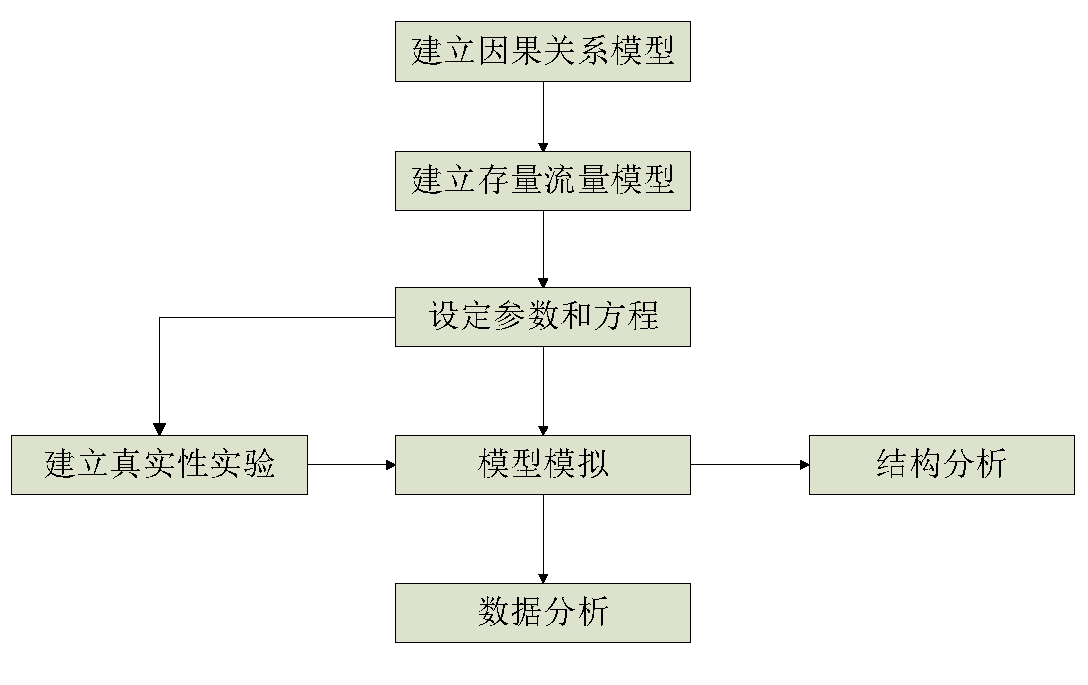
\includegraphics{vensim.pdf}}
  \caption{模型仿真过程}
  \label{fig:vensim}
\end{figure}
\subsection{动机因素存量流量图}

在因果图中,不论是动机因素,还是个体的行为都是系统的状态,是存量。为了
描述动机于行为间的关系而故意忽略了一些流量变量和外生变量。但是,这些被
忽略的变量对于整个系统起到了重要作用,没有这些变量系统就不可能正确地表
示现实系统的运行。

对于大部分动机因素,它们和个体的行为之间构成了一个正反馈回路和一个负反
馈回路,既动机的
增强会提升个体的行为水平,如果协同行为的得到了他人的正反馈,则会提升个体的动
机;反之如果协同行为得到了他人的负反馈,个体的动机会受到伤害。对于现实
系统来说,有几个重要的变量未能包含在因果图中。首先,个体的协同行为水平
不仅受到动机的影响,还受到其他因素,尤其是个体工作能力的限制。无论个体怎么
提升协同水平,都不可能超过个体的最大工作能力。这就是所谓“增长的极限”。
个体的最大工作能力是行为水平的抑制因素,使得行为水平不可能无限制地增长
下去。其次,动机作为系统中的存量,必然要受到流量的影响。动机的流
入是从协同活动中获得的正反馈转化的动机,动机的流出则是协同活动中获得的
负反馈使动机削弱的数量。流入水平和流出水平综合决定了动机存量的变化。第
三,不论是动机转化为行为还是行为的结果反馈影响动机都不是线性过程。这种
变换也存在遍及递减效应,动机的水平越高,每增加一单位动机所能引起的行为
水平的增加就越少。因此如果仅考虑行为与动机的互动关系的话,个体的动机应
该呈对数增长(或减弱),最后接近某个极大(小)值。最后,成就动机同其他
动机略有不同。成就动机促使个体参与某种活动从中获得成就感。成就感的提升
削弱成就需求。但是成就感有一种随时间自动削弱的属性,在没有任何外力介入
的情况下成就感将逐渐流失,从而提升了个体的成就需求,促使他们参与新的活
动重新获得成就感。流失速度的不同决定了不同人的行为模式,对于流失速度快
的人来说,他们从参与活动中所获得的成就感迅速减少,因此这些人表现为进取
精神非常强,不停地追逐新的目标来满足自己对成功的渴望。而流失速度慢的人则
会很长时间满足于自身取得的成就,表现为为止步不前,不愿接受新的挑战。

根据以上分析的结果,本文将把因果关系图转换为存量流量图,同时在模型中加
入新的变量,使模型更符合现实世界。因为转换的模型力图完整描述存量于流量
的关系,因此对因果关系进行了简化处理。变量间具体、详细的因果关系请参考
因果关系图。大部分的动机因素都有同样的特征:动机增加引起行为水平的提升;
如果行为得到正反馈则会促使动机也得到相应的提升,负反馈则会使动机减弱。
因此将这一类动机合并表示一般动机。对于利他主义和感知到的意义两类动机由
于和行为之间是单向关系,统称为无反馈动机。成就动机和认知失调两类动机有
各自的特点,所以单独保留。引入了流量变量“每次协同行为增加的动机”表示
动机的流入,“他人对个体的协同行为减少的动机”表示动机的流出,以此表示
动机的动态性;引入变量“疲劳“和外生变量“个人工作的最大能力”构建行为
的负反馈闭环,反应行为水平受到抑制的特征。引入流量变量“满足感的流失”
反应满足感随时间减少的特点。转换的存量流量图如图
\ref{fig:refined-model}所示。
\begin{figure}[htb]
  \centering
  \scalebox{0.7}{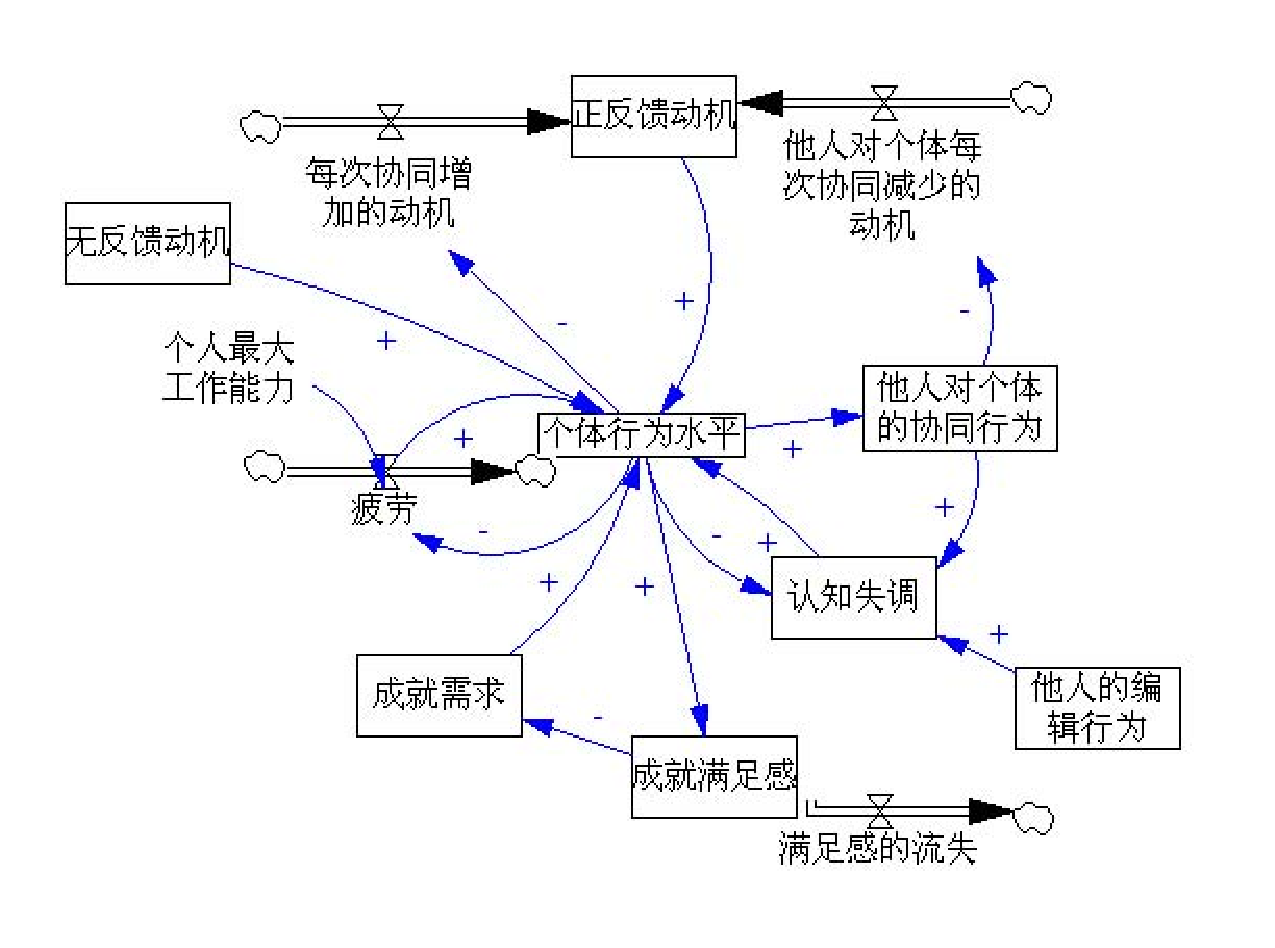
\includegraphics{refinedmodel1.pdf}}
  \caption{\small{知识协同动机因素的存量流量图}}
  \label{fig:refined-model}
\end{figure}

\subsection{模型方程的设置}

每个变量都和其他变量形成一定的函数关系,这种关系使用方程来表示。下面列
举了了模型中所有涉及到的方程。
\begin{enumerate}
\item 行为水平=转换水平$\times (\sum$一般动机+成就动机+认知失调+无反馈
  动机)
\item 成就需求=个体的最大成就需求-满足感$\times$转换系数
\item 自我决定=上一期自我决定+正协同贡献$\times$转换系数+负协同贡献
  $\times$转换系数
\item  自我效能=上一期自我效能+正协同贡献$\times$转换系数+负协同贡献
  $\times$转换系数
\item 自我肯定=上一期自我肯定+正协同贡献$\times$转换系数+负协同贡献
  $\times$转换系数
\item 认知失调=他人的协同行为$\times$转换系数+他人对个体的协同行为
  $\times$转换系数-协同行为水平$\times$转换系数
\item 群体效能=上一期群体效能定+正协同贡献$\times$转换系数+负协同贡献
  $\times$转换系数
\item 归属感=上一期归属感+正协同贡献$\times$转换系数+负协同贡献
  $\times$转换系数
\item 自我决定到协同水平的转换系数
\item 自我效能到协同水平的转换系数
\item 自我肯定到协同水平的转换系数
\item 成就需求到协同水平的转换系数
\item 认知失调到协同水平的转换系数
\item 群体效能到协同水平的转换系数
\item 归属感到协同水平的转换系数
\item 正协同贡献到自我决定的转换系数
\item 正协同贡献到自我效能的转换系数
\item 正协同贡献到自我肯定的转换系数
\item 正协同贡献到成就需求的转换系数
\item 正协同贡献到认知失调的转换系数
\item 正协同贡献到群体效能的转换系数
\item 正协同贡献到归属感的转换系数
\item 负协同贡献到自我决定的转换系数
\item 负协同贡献到自我效能的转换系数
\item 负协同贡献到自我肯定的转换系数
\item 负协同贡献到成就需求的转换系数
\item 负协同贡献到认知失调的转换系数
\item 负协同贡献到群体效能的转换系数
\item 负协同贡献到归属感的转换系数

\end{enumerate}

\subsection{参数估计}
参数估计是建立系统动力学模型重要的过程。即使是参数值的微小变化,也可能会引起系统
行为产生较大幅度的波动,甚至改变整个系统行为的极
性。因此, 为保证模型模拟结果与真实系统的一致性, 应尽可能地准确估计模型
的参数。

模型的参数估计是模型的局部分别独立地进行,然后在总体模型进行模拟仿真时
在进行总的调试。系统动力学本身并不限制参数估计的方法,可以根据需要和具
体情况灵活地选用不同的参数估计方法。参数估计的完成标志着模型从定性向定
量的转化。

参数的估计方法可以分为以下几种。
目前SD 模型参数估计的技术大致可分为3 种[1, 2 ]: (1) 单个参数、表函数关系、间接计算等基于利用
模型变量集结程度以下的数据进行的估计; (2) 运用单方程进行估计; (3) 运用多方程进行估计等. 其中后
2 种都是基于与模型变量集结程度相当的数据进行的估计. 此外, 还可以运用统计技术进行估计.
但是, SD 模型基于结构而不是统计相关性的特征, 使得它所要求的许多参数(如国民经济系统中描述
人均国民收入对积累率影响程度的参数等) 往往缺乏可资利用的资料, 使建模工作者可以有效地运用前述
的种种方法对它们进行合理的估计. 还有一种情况, 由于SD 模型所处理的常是具有多重反馈的复杂系
统, 这使得处在因果链上相隔甚远的变量间的关系变得很不直观甚至反直观, 要估计描述它们对应关系的
参数也十分困难. 为了对这些难以估计的参数进行估计, 有时就得采用“仿真—分析—修正”这种类似于手
工式的“试凑法'' \cite{linwenhao2002}。

参数的估计工作分为两部分,一部分是估计变量的初值,另一部分是估计方程中
的参数。在动机因素于协同行为的模型中,大部分变量都是定性变量,本身就难
于量化。在缺乏资料的情况下,将定性变量数量化,本身就带有一定的盲目性和
随意性,因此手工调试是必不可少的环节。但是,通过使用一定的估计方法能大
大简化手工调试的工作量,减少调试的时间。


\begin{table}[htb]
  \centering
\small
% Table generated by Excel2LaTeX from sheet 'Sheet2'
\begin{tabular}{|r|r|r|r|r|r|}
\hline
\multicolumn{ 1}{|c|}{变量名称} &                                     \multicolumn{ 5}{|c|}{初始值} \\
\hline
\multicolumn{ 1}{|c|}{} &        领导者 &       领域专家 &      内容贡献者 &      内容维护者 &       边缘用户 \\
\hline
      利他主义 &            &            &            &            &            \\
\hline
    感知到的意义 &            &            &            &            &            \\
\hline
      自我决定 &            &            &            &            &            \\
\hline
      自我效能 &            &            &            &            &            \\
\hline
      自我肯定 &            &            &            &            &            \\
\hline
      成就需求 &            &            &            &            &            \\
\hline
      认知失调 &            &            &            &            &            \\
\hline
      群体效能 &            &            &            &            &            \\
\hline
       归属感 &            &            &            &            &            \\
\hline
     满足感流失 &            &            &            &            &            \\
\hline
自我决定到协同水平的转换系数 &            &            &            &            &            \\
\hline
自我效能到协同水平的转换系数 &            &            &            &            &            \\
\hline
自我肯定到协同水平的转换系数 &            &            &            &            &            \\
\hline
成就需求到协同水平的转换系数 &            &            &            &            &            \\
\hline
认知失调到协同水平的转换系数 &            &            &            &            &            \\
\hline
群体效能到协同水平的转换系数 &            &            &            &            &            \\
\hline
归属感到协同水平的转换系数 &            &            &            &            &            \\
\hline
正协同贡献到自我决定的转换系数 &            &            &            &            &            \\
\hline
正协同贡献到自我效能的转换系数 &            &            &            &            &            \\
\hline
正协同贡献到自我肯定的转换系数 &            &            &            &            &            \\
\hline
正协同贡献到成就需求的转换系数 &            &            &            &            &            \\
\hline
正协同贡献到认知失调的转换系数 &            &            &            &            &            \\
\hline
正协同贡献到群体效能的转换系数 &            &            &            &            &            \\
\hline
正协同贡献到归属感的转换系数 &            &            &            &            &            \\
\hline
负协同贡献到自我决定的转换系数 &            &            &            &            &            \\
\hline
负协同贡献到自我效能的转换系数 &            &            &            &            &            \\
\hline
负协同贡献到自我肯定的转换系数 &            &            &            &            &            \\
\hline
负协同贡献到成就需求的转换系数 &            &            &            &            &            \\
\hline
负协同贡献到认知失调的转换系数 &            &            &            &            &            \\
\hline
负协同贡献到群体效能的转换系数 &            &            &            &            &            \\
\hline
负协同贡献到归属感的转换系数 &            &            &            &            &            \\
\hline
\end{tabular}  

  \caption{\small{参数初始值}}
  \label{tab:initail-value}
\end{table}

\section{模型检验}

当模型的所有参数都确定后,需要测试模型的有效性,检查模型是否能较准确地
模拟现实系统。模型的检验是一个不断证伪的过程。常见的检验方法包括结构评
价测试、参数估计测试、行为重现测试、灵敏度测试、系统改进测试等。检验往
往是通过同用户、专家的不断对话,深入理解系统行为,同时检查系统的因果关
系是否合理,方程量纲是否一致,对模型进行各种条件下的测试,并对比模型的
运行结果和实际数据。本文在参考大量文献的基础上,借鉴了其他学者的实证研
究成果,对模型进行直观检验,观测模型是否能重现真实系统中的行为变化。

模型是现实世界的简化和抽象,因此一个模型不可能精确地再现现实中的各种现
象。模型的主要目的在于反映趋势的变化。为了验证模型的正确性,本文将模型
仿真数据同真实数据进行对比。针对不同类型的用户,使用维基百科提供的数据分别计算了连续40个月的
月人均贡献度和仿真结果进行比对。

图\ref{fig:simu1}是领导者用户的仿真结果和真实数据图。从图中可以看出,领导者用户的月人
均贡献度呈现出比较明显的对数函数特征,而仿真的结果显示为系统行为呈现出
寻的模式,因此虽然模型同实际数据有误差,但是仍然较准确地再现了现实趋
势,可以使用模型模拟用户的知识协同行为。

\begin{figure}[!htb]
  \centering
  \scalebox{0.76}{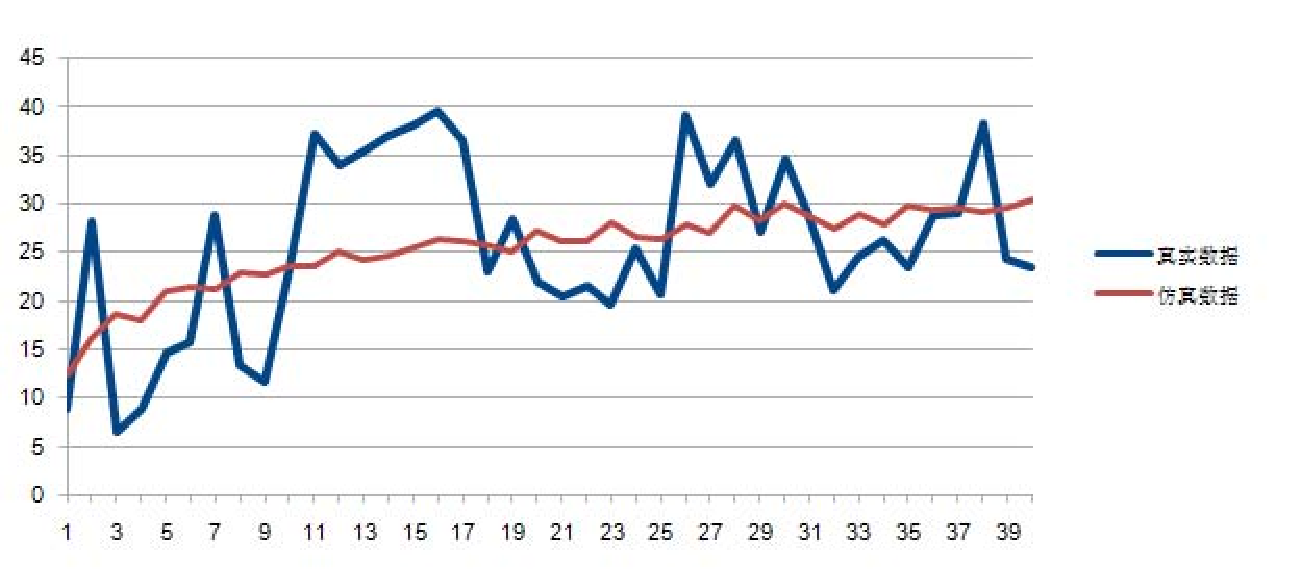
\includegraphics{simu-1.pdf}}
  \caption{\small{领导者用户仿真结果}}
  \label{fig:simu1}
\end{figure}

图\ref{fig:simu2}是领域专家用户的仿真结果和真实数据图。真实数据反映出该类用户的月人均
贡献度在初期显著下降后迅速进入一个平稳状态。仿真结果则表现为一个递减
的对数函数。两者的趋势是一致的。

\begin{figure}[!htb]
  \centering
  \scalebox{0.69}{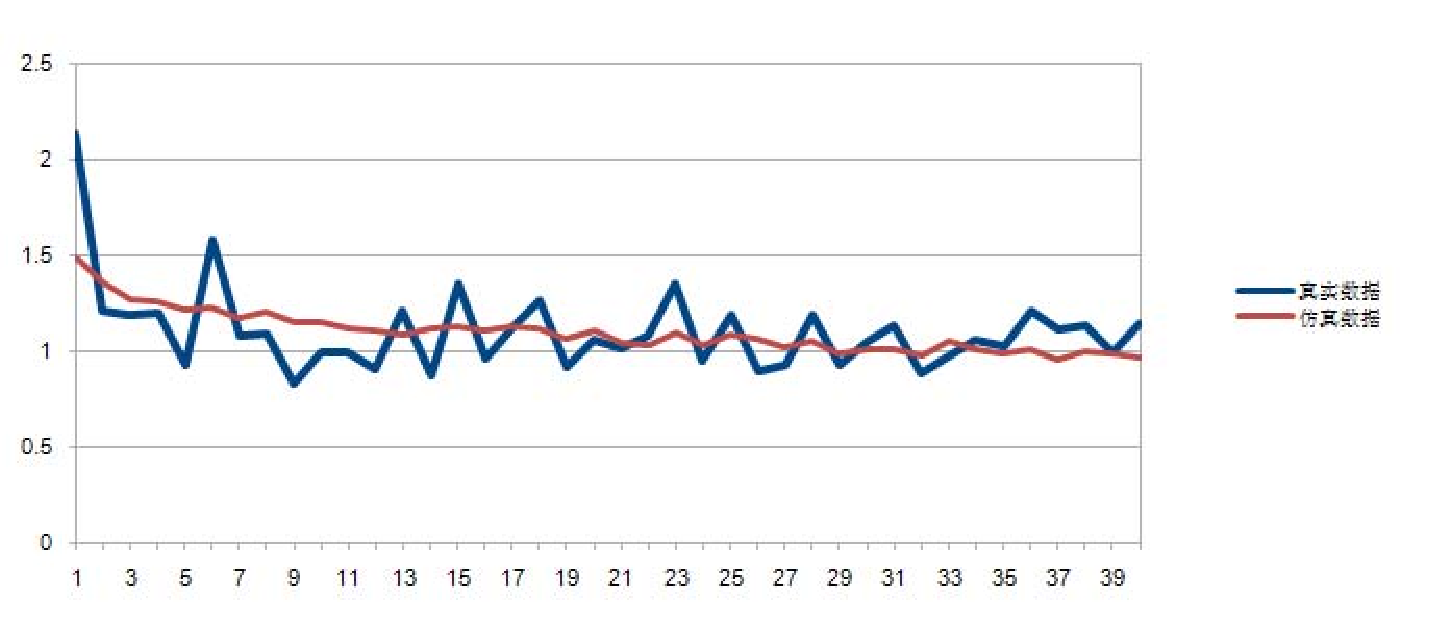
\includegraphics{simu-2.pdf}}
  \caption{\small{领域专家用户仿真结果}}
  \label{fig:simu2}
\end{figure}

图\ref{fig:simu3}是内容贡献者的仿真结果和真实数据图。内容贡献者的月人均
贡献度非常平稳,没有明显的震荡。仿真的结果也几乎是一条直线,同实际数据
的拟合度很高。因此模型很好地反映了内容贡献者的动机与知识协同水平的相互
作用。

\begin{figure}[!htb]
  \centering
  \scalebox{0.76}{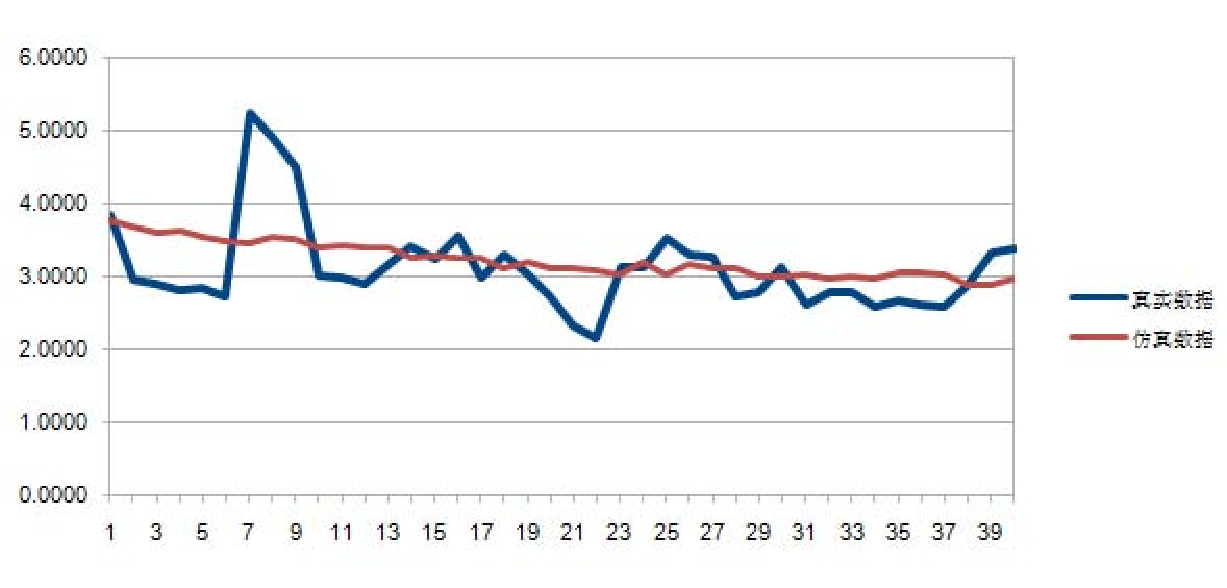
\includegraphics{simu-3.pdf}}
  \caption{\small{内容维护者用户仿真结果}}
  \label{fig:simu3}
\end{figure}

图\ref{fig:simu4}是内容维护者的仿真结果和真实数据图。实际数据显示内容
维护者的月人均贡献很快下滑,随后逐渐平稳,下滑趋势减缓。仿真数据则是一
条对数曲线,除了和个别真实点的数据结果差距很大以外,整体的拟合度很高,
说明模型对于分析内容维护者的行为是有效的。
\begin{figure}[!htb]
  \centering
  \scalebox{0.76}{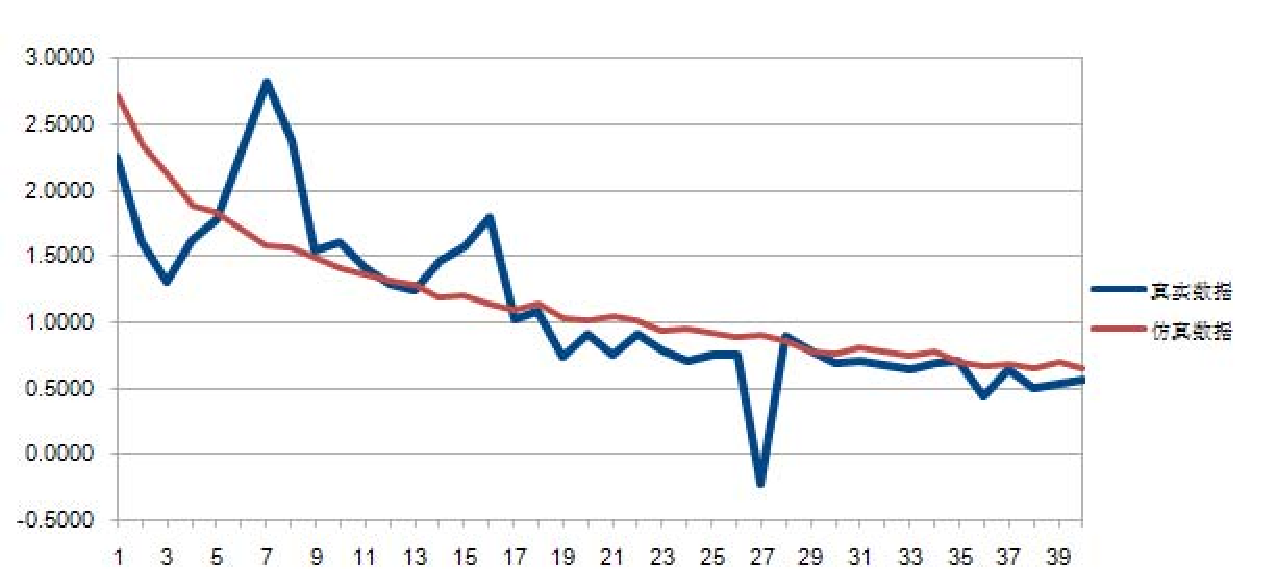
\includegraphics{simu-4.pdf}}
  \caption{\small{内容贡献者用户仿真结果}}
  \label{fig:simu4}
\end{figure}

图\ref{fig:simu5}是边缘用户的仿真结果和真实数据图。边缘用户的月人均贡
献值是所有用户类型中最为特殊的:呈加速下滑趋势。模型仿真结果也显示月人均贡献是一条近
似于指数函数的曲线。虽然真实数据的波动水平比较大,但是模型的拟合结果仍
然反映了真实系统的变动趋势。
\begin{figure}[!htb]
  \centering
  \scalebox{0.76}{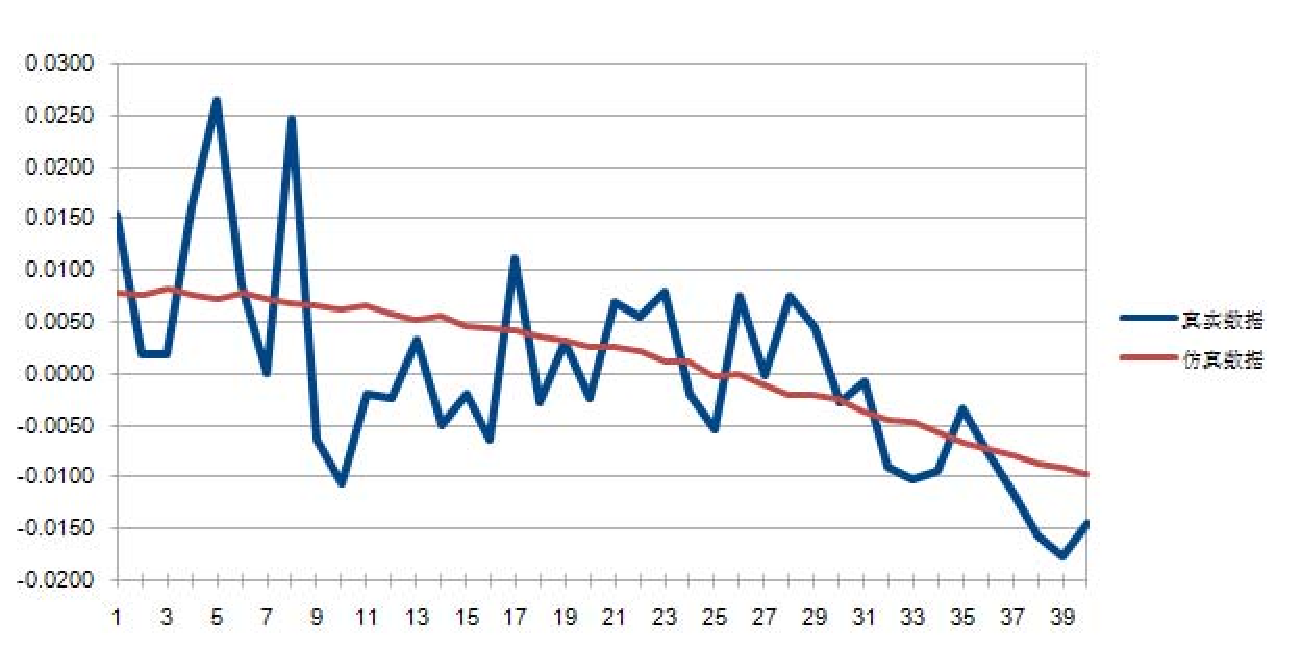
\includegraphics{simu-5.pdf}}
  \caption{\small{边缘用户仿真结果}}
  \label{fig:simu5}
\end{figure}

%%% Local Variables: 
%%% mode: latex
%%% TeX-master: t
%%% End: 
